\documentclass[12pt,a4paper,bibliography=totocnumbered,listof=totocnumbered]{scrartcl}
\usepackage[ngerman]{babel}
\usepackage[utf8]{inputenc}
\usepackage{amsmath}
\usepackage{amsfonts}
\usepackage{amssymb}
\usepackage{graphicx}
\usepackage{fancyhdr}
\usepackage{tabularx}
\usepackage{geometry}
\usepackage{setspace}
\usepackage[right]{eurosym}
\usepackage{subfig}
\usepackage{floatflt}
\usepackage[usenames,dvipsnames]{color}
\usepackage{colortbl}
\usepackage{paralist}
\usepackage{array}
\usepackage{titlesec}
\usepackage{parskip}
\usepackage[right]{eurosym}
\usepackage[subfigure,titles]{tocloft}
\usepackage[pdfpagelabels=true]{hyperref}
\usepackage{amsthm}
\usepackage{listings}
\usepackage{mdframed}
\usepackage{pdfpages}
\usepackage{breqn}

\usepackage{url}
\def\UrlBreaks{\do\/\do-}

\newtheorem{definition}{Definition}
\newtheorem{claim}{Behauptung}
\newtheorem{theorem}{Satz}
\newtheorem{protocol}{Protokoll}
\newtheorem{algorithm}{Algorithmus}

\lstset{basicstyle=\footnotesize, captionpos=b, breaklines=true, showstringspaces=false, tabsize=2, frame=lines, numbers=left, numberstyle=\tiny, xleftmargin=2em, framexleftmargin=2em}
\makeatletter
\def\l@lstlisting#1#2{\@dottedtocline{1}{0em}{1em}{\hspace{1,5em} Lst. #1}{#2}}
\makeatother

\geometry{a4paper, top=27mm, left=30mm, right=20mm, bottom=35mm, headsep=10mm, footskip=12mm}

\hypersetup{
  unicode=false,
  pdftoolbar=true,
  pdfmenubar=true,
  pdffitwindow=false,
  pdfstartview={FitH},
  pdftitle={Zero Knowledge Proofs},
  pdfauthor={Konstantin Fickel},
  pdfsubject={Seminararbeit Zero Knowledge},
  pdfcreator={\LaTeX},
  pdfproducer={pdfTeX \the\pdftexversion.\pdftexrevision},
  pdfkeywords={Seminararbeit},
  pdfnewwindow=true,
  colorlinks=true,
  linkcolor=black,
  citecolor=black,
  filecolor=magenta,
  urlcolor=black
}
\pdfinfo{/CreationDate (D:20170705000000)}

\begin{document}


\includepdf[pages={1}]{img/cover.pdf}

\titlespacing{\section}{0pt}{12pt plus 4pt minus 2pt}{-6pt plus 2pt minus 2pt}

% Kopf- und Fusszeile
\renewcommand{\sectionmark}[1]{\markright{#1}}
\renewcommand{\leftmark}{\rightmark}
\pagestyle{fancy}
\lhead{}
\chead{}
\rhead{\thesection\space\contentsname}
\lfoot{Zero Knowledge}
\cfoot{}
\rfoot{\ \linebreak Seite \thepage}
\renewcommand{\headrulewidth}{0.4pt}
\renewcommand{\footrulewidth}{0.4pt}

% Vorspann
\renewcommand{\thesection}{\Roman{section}}
\renewcommand{\theHsection}{\Roman{section}}
\pagenumbering{Roman}

% ----------------------------------------------------------------------------------------------------------
% Titelseite
% ----------------------------------------------------------------------------------------------------------
\thispagestyle{empty}
\begin{center}
	
\includegraphics[scale=0.22]{img/00_logo_unia.pdf}\\
	\vspace*{2cm}
	\Large
	\textbf{Fakultät}\\
	\textbf{Angewandte Informatik}\\
	\vspace*{2cm}
	\Huge
	\textbf{Seminararbeit}\\
	\vspace*{0.5cm}
	\large
	über das Thema\\
	\vspace*{1cm}
	\textbf{Zero Knowledge}\\
	\vspace*{2cm}
      
	\vfill
	\normalsize
	\newcolumntype{x}[1]{>{\raggedleft\arraybackslash\hspace{0pt}}p{#1}}
	\begin{tabular}{x{3.5cm}p{10cm}}
		\rule{0mm}{5ex}\textbf{Autor:} & Konstantin Fickel\newline konstantin.fickel@student.uni-augsburg.de \\ 
		\rule{0mm}{5ex}\textbf{Betreuer:} & Kuzman Katkalov \\ 
		\rule{0mm}{5ex}\textbf{Abgabedatum:} & 05. 07. 2017 \\ 
	\end{tabular} 
\end{center}
\pagebreak

% ----------------------------------------------------------------------------------------------------------
% Abstract
% ----------------------------------------------------------------------------------------------------------
\setcounter{page}{1}
\onehalfspacing
\titlespacing{\section}{0pt}{12pt plus 4pt minus 2pt}{2pt plus 2pt minus 2pt}

\pagebreak

% ----------------------------------------------------------------------------------------------------------
% Verzeichnisse
% % ----------------------------------------------------------------------------------------------------------
% TODO Typ vor Nummer
\renewcommand{\cfttabpresnum}{Tab. }
\renewcommand{\cftfigpresnum}{Abb. }
\settowidth{\cfttabnumwidth}{Abb. 10\quad}
\settowidth{\cftfignumwidth}{Abb. 10\quad}

\titlespacing{\section}{0pt}{12pt plus 4pt minus 2pt}{2pt plus 2pt minus 2pt}
\singlespacing
\rhead{INHALTSVERZEICHNIS}
\renewcommand{\contentsname}{Inhaltsverzeichnis}
\phantomsection
\addtocounter{section}{1}
\tableofcontents

\pagebreak

% ----------------------------------------------------------------------------------------------------------
% Inhalt
% ----------------------------------------------------------------------------------------------------------
% Abstände Überschrift
% \titlespacing{\section}{0pt}{12pt plus 4pt minus 2pt}{-6pt plus 2pt minus 2pt}
% \titlespacing{\subsection}{0pt}{12pt plus 4pt minus 2pt}{-6pt plus 2pt minus 2pt}
% \titlespacing{\subsubsection}{0pt}{12pt plus 4pt minus 2pt}{-6pt plus 2pt minus 2pt}

% % Kopfzeile
\renewcommand{\sectionmark}[1]{\markright{#1}}
\renewcommand{\subsectionmark}[1]{}
\renewcommand{\subsubsectionmark}[1]{}
\lhead{Kapitel \thesection}
\rhead{\rightmark}

\onehalfspacing
\renewcommand{\thesection}{\arabic{section}}
\renewcommand{\theHsection}{\arabic{section}}
\setcounter{section}{0}
\pagenumbering{arabic}
\setcounter{page}{1}

% ----------------------------------------------------------------------------------------------------------
% Einleitung
% ----------------------------------------------------------------------------------------------------------
\section{Einleitung}

Nach seinen Enthüllungen der illegalen Aktivitäten der amerikanischen Geheimdienste im Jahr 2013 galt der Whistleblower Edward Snowden auch als eine Art Autorität für Datenschutz. So wurde darüber berichtet, dass Snowden in einem Guardian-Interview von einer Verwendung von Diensten wie Dropbox warnte, da diese die in der Cloud gespeicherten Daten lesen und auswerten können. Er empfahl, stattdessen einen \glqq{}Zero Knowledge\grqq{}-Anbieter wie Spideroak zu verwenden.\footnote{siehe \cite{snowden}} Damit meinte er eine konsequente Verschlüsselung und Entschlüsselung der Daten auf dem Gerät des Nutzers mit einem Schlüssel, auf den den der Cloud Provider keinen Zugriff besitzt. So kann der Cloudspeicheranbieter auch nicht auf die Daten zugreifen und diese analysieren - womit er \glqq{}nichts weiß\grqq{}.

Spätestens ab diesem Zeitpunkt richtete sich die öffentliche Aufmerksamkeit auf den Begriff \glqq{}Zero Knowledge\grqq{}. Spideroaks Verständnis desselben deckt sich jedoch nicht ganz mit der mathematischen Definition, oder genauer mit Zero-Knowledge-Beweisprotokollen, mit denen sich diese Arbeit beschäftigen wird. Dabei geht es um einen Beweiser, der die Lösung eines (mathematischen) Problems kennt, und einen Verifizierer, den dieser davon überzeugen soll, dass er im Besitz der Lösung ist. Der Verifizierer darf jedoch, unabhängig davon, was er versucht, kein zusätzliches Wissen zur Lösung des Problems aus der Konversation bekommen. 

Dies wurde auch dem \glqq{}Zero Knowledge\grqq{}-Anbieter Spideroak klar, sodass er um den Unterschied seines Produktes zur mathematischen Variante zu verdeutlichen am Anfang dieses Jahres auf seiner Website den Begriff zu \glqq{}No Knowledge\grqq{} änderte.\footnote{siehe \cite{noknowledge}}

Doch zurück zu den mathematischen Zero-Knowledge-Beweisen: Deren Konzept wurde erstmalig von Schafi Goldwasser, Silvio Micali und Charles Rackoff eingeführt. Die ersten Versionen der Arbeit darüber entstanden bereits im Jahr 1982. Jedoch wurde diese von drei größeren Konferenzen abgelehnt, bis sie schließlich im Jahr 1995 im Rahmen der \glqq{}Symposium on Theory of Computing\grqq{}, einer wissenschaftlichen Konferenz für theoretische Informatik, erstmalig publiziert wurde. Die Anwendung auf viele Probleme wurde von Oded Goldreich, Silvio Micali und Widgerson erschlossen, die zeigen konnten, dass sich für jede Sprache in NP ein Zero-Knowledge-Beweis konstruieren lässt.\footnote{aus \cite[Seite 3]{20yearszeroknowledge}}

In den folgenden Abschnitten werde ich Zero Knowledge formal definieren, zwei eher theoretische Beispiele präsentieren, erläutern, wie man für jede Sprache in NP einen Zero-Knowledge-Beweis konstruieren kann und anschließend verschiedene praktische Anwendungen von Zero Knowledge wie Zcash und ein Authentifizierungsprotokoll vorstellen.

\pagebreak


\section{Definition}
Um einen Zero-Knowledge-Beweis definieren zu können, muss man sich erst einmal auf eine konkrete Definition eines Beweises festlegen. Im allgemeinen mathematischen Ver\-ständ\-nis ist dieser eine von einem Beweiser aufgeschriebene statische Zeichenkette \( \pi \), in dem eine Aussage mithilfe von Axiomen und Schlussregeln so hergeleitet wird, dass jeder Verifizierer sich selbst von der Korrektheit der Aussage überzeugen kann.

\cite{goldwasser1989} verallgemeinert den Beweisbegriff: Zum einen wird Interaktion zugelassen, das heißt, der Verifzierer \( V \) kann dem Beweiser \( P \) Fragen stellen, auf die jener antworten kann. Außerdem muss der Verifizierer nicht mit letzter Sicherheit überzeugt sein, es genügt, wenn dieser mit einer sehr hohen Sicherheit (von beispielsweise \( 99,9  \% \)) von der Aussage überzeugt werden kann.\footnote{vgl. \cite[Seite 2]{princeton}}
 
\subsection{Interaktive Protokolle}

Wie kann man aber so ein Beweissystem formal fassen? Hierzu werden die einzelnen Teilnehmer als eine Erweiterung einer normalen Turing-Maschine festgelegt. Das Alphabet der Sprachen (hier bezeichnet mit  dem Symbol \( L \)) sei in der gesamten Arbeit \( \Sigma = \left\lbrace 0, 1 \right\rbrace \).

% TODO: Abstand
\vspace{0.2cm}

\begin{definition}[Interaktive Turing-Maschine]
Eine Interaktive Turing Maschine (kurz ITM) ist eine Sechs-Band-Turing-Maschine mit einem \textnormal{Arbeitsband}, einem nur-lesbaren \glqq{}öffentlichen\grqq{} \textnormal{Eingabeband},einem nur-lesbaren \glqq{}privaten\grqq{} Eingabeband, jeweils einem nur-les- bzw. nur-beschreibbaren \textnormal{Kommunikationsband} und einem \textnormal{Zufallszahlenband}, das mit Zufallsbits beschrieben ist.\footnote{vgl. \cite[Definition 1.1]{np}, \cite[Abschnitt 2.1]{goldwasser1989} und geheimes Eingabeband aus \cite[Chapter 2]{identity}}
\end{definition}

Zwei solcher Automaten gemeinsam können dann ein Protokoll beschreiben:

% TODO: Abstand
\vspace{0.2cm}

\begin{definition}[Interaktives Protokoll]
Ein interaktives Protokoll ist ein geordnetes Paar \( \left< P, V \right> \) zweier ITMs, die sich das \glqq{}öffentliche\grqq{} Eingabeband teilen und jeweils das beschreibbare Kommunikationsband der einen das lesbare Kommunikationsband der anderen ITM ist. Beide Maschinen führen ihre Berechnung abwechselnd durch: Während die eine rechnet, befindet sich die andere im \glqq{}Leerlauf\grqq{}. Das Wort, das von einer während eines einzelnen Berechnungsschrittes auf das Band geschrieben wird, wird als die zur anderen ITM \textnormal{gesendete Nachricht} bezeichnet.\footnote{vgl. \cite[Abschnitt 2.1]{goldwasser1989} und \cite[Definition 1.3]{np}}
\end{definition}

Die beiden interaktiven Turing-Maschinen \( \left< P, V\right> \) sind hier das Modell für den Beweiser \( P \) und den Verifizierer \( V \). Eine Kommunikation der beiden probabilistischen Maschinen mit der gemeinsamen Eingabe \( \omega \) kann auch als Zufallsvariable \( \left< P, V \right> \left( \omega \right) \) aufgefasst werden.

\vspace{1em}
\begin{minipage}{\linewidth}
	\centering
	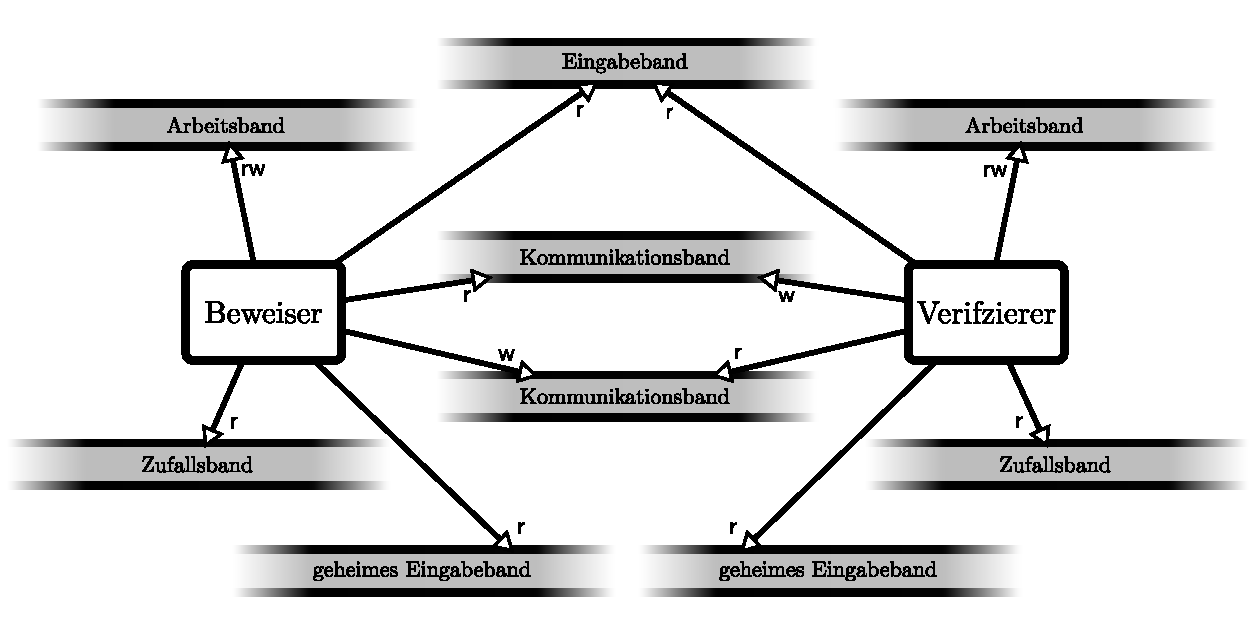
\includegraphics[width=0.9\linewidth]{img/interactiveprotocol.pdf}
	\captionof{figure}[Interaktives Protokoll]{Interaktives Protokoll mit Beweiser \( P \) und Verifizierer \( V \)}
	\label{fig:interactiveprotocol}
\end{minipage}

% TODO: Abstand
\vspace{0.2cm}

\begin{definition}[Interaktive Beweissysteme]
\label{definition:proofsystem}
Ein interaktives Beweissystem ist ein interaktives Protokoll 
\( \left< P, V\right> \). Dabei ist die Laufzeit von \( V \) und \( P \) polynomiell bezüglich des Wortes auf dem Eingabeband beschränkt. Das geheime Eingabeband des Beweisers beinhaltet die Lösung des Problems, das des Verifizierers bleibt leer. Zusätzlich sei erfüllt:\footnote{In den meisten Werken zu dem Thema (wie z.B. \cite{np}) kann der Beweiser eine unbegrenzte Laufzeit besitzen und hat dafür kein geheimes Eingabeband. Da in keinem der hier besprochenen Beispielen dies benötigt wird, habe ich mich stattdessen für eine polynomielle Laufzeit und ein geheimes Eingabeband entschieden. Siehe \cite[Chapter 2]{identity}, \cite[Definition 1]{20yearszeroknowledge} und \cite[Definition 2]{np}}
\begin{itemize}

\item[\textnormal{Vollständigkeit:}] \( \forall \omega \in L : \textnormal{\textbf{\textsf{P}}} \left( V \textnormal{ akzeptiert bei } \left< P, V \right> \left( \omega \right) \right) = 1 \)  \glqq{}Für jedes \( \omega \in L \) akzeptiert \( V \) immer nach der Durchführung des Beweises mit dem Beweiser \( P \).\grqq{}

\item[\textnormal{Korrektheit:}] \( \exists p \textnormal{ Polynom}: \forall \omega \notin L, P^{\ast} \textnormal{ beliebige ITM} : \textnormal{\textbf{\textsf{P}}} \left( V \textnormal{ akzeptiert bei } \left< P ^{\ast}, V \right> \left( \omega \right) \right) \leq \frac{1}{p \left( \left| \omega \right| \right)}  \) \glqq{}Für jedes \( \omega \notin L \) gibt es keine Strategie, mit der der Verfizierer \glqq{}immer\grqq{} überzeugt werden kann.\grqq{}
\end{itemize}
\end{definition}

 Falls \( V \) akzeptiert (also überzeugt werden konnte) oder verwirft, vermerkt er dies auf seinem Kommunikationsband und beendet das Protokoll.

\subsection{Zero Knowledge}
Informell bedeutet Zero Knowledge, dass egal, was der Verifizierer versucht, er keine zusätzlichen Informationen aus dem Beweiser bekommen kann, die er sich mit seiner polynomiellen Beschränkung nicht hätte selbst berechnen können. Dies wird hier durch einen ebenfalls im Erwartungswert polynomiellen Simulator definiert, der den Verfizierer bekommt und anhand dessen eine mögliche Kommunikation zwischen diesem Verifizierer und dem im Protokoll spezifizierten Beweiser ausgibt, welche für einen polynomiellen Algorithmus ununterscheidbar von einer echten Kommunikation ist. Dabei soll es egal sein, ob der Verifizierer \textit{ehrlich} ist, sich also an das Protokoll hält, oder ob er bewusst versucht, durch falsche Eingaben den Beweiser zu für ihn nützlichen Aussagen zu bringen.

Was hier noch für die vollständige Definition von Ze ro Knowledge fehlt, ist eine Möglichkeit auszusagen, dass sich zwei verschiedene Zufallsvariablen genug ähneln, sodass diese für eine polynomiell beschränkte Turing-Maschine nicht unterscheidbar sind.

% TODO: Abstand
\vspace{0.2cm}

\begin{definition}[Rechnerische Ununterscheidbarkeit] Sei \( L \) eine Sprache.
Zwei in der Länge polynomiell beschränkte Zufallsvariablen \( U \left( \omega \right) \) und \( V \left( \omega \right) \) über \( L \) sind rechnerisch ununterscheidbar, falls für jeden im Erwartungswert polynomiellen Algorithmus \( C \) und für jedes Polynom \( p \) bei ausreichend langem \( \omega \in L \) gilt:\footnote{vgl. \cite[Seite 93]{goldwasser1989}}
\[ \left| \textnormal{\textbf{\textsf{P}}} \left( C \left( U \left( \omega \right) \right) = 1 \right) - \textnormal{\textbf{\textsf{P}}} \left( C \left( V \left( \omega \right) \right) = 1 \right) \right| < \frac{1}{p \left( \left| \omega \right| \right)} \]
\end{definition}

Da man das Ergebnis nicht-deterministischer Berechnungen als Zufallsvariable auffassen kann, lässt sich nun Zero Knowledge definieren:

% TODO: Abstand
\vspace{0.2cm}

\begin{definition}[Zero Knowledge]
\label{definition:zeroknowledge}
Ein Beweiser \( P \) ist genau dann (rechnerisch) \textnormal{Zero Knowledge} auf Eingabewörtern aus \( L \), wenn für jeden probabilistisch-polynomiellen Verifizierer \( V ^ {\ast} \) eine im Erwartungswert polynomielle Turing-Maschine \( M_{V^{\ast}} \) existiert, die die Kommunikation zwischen \( P \) und \( V^{\ast} \) simuliert, sodass folgende Familien von Zufallsvariablen rechnerisch ununterscheidbar sind:\footnote{vgl. \cite[Definition 4]{20yearszeroknowledge}}
\begin{enumerate}
\item[1.] \( \left\lbrace \left< P, V^{\ast} \right> \left( \omega \right) \right\rbrace _{\omega \in L} \) \( \overset{\textnormal{def}}{=} \) die Kommunikation zwischen \( V ^ {\ast}\) und \( P \) bei gemeinsamer Eingabe \( \omega \in L \).
\item[2.] \( \left\lbrace M_{V^{\ast}} \left( \omega \right) \right\rbrace _{\omega \in L} \) \( \overset{\textnormal{def}}{=} \) die Ausgabe des Simulators \( M_{V^{\ast}} \) bei der Eingabe von \( \omega \in L \). 
\end{enumerate}
\end{definition}

\pagebreak


\section{Beispiele für Zero-Knowledge-Beweise}

\subsection{Graphenisomorphismus}
\begin{definition}[Graphenisomorphismus]
Gegeben seien zwei Graphen \( G_0 = \left( V_0, E_0 \right) \) und \( G_1 = \left( V_1, E_1 \right) \). Beide Graphen sind genau dann isomorph zueinander, wenn man einen Graphen durch Umbenennung der Knoten in den anderen umwandeln kann. Die Sprache der isomorphen Graphen ist somit

\[ L_{isomorph} = \left\lbrace \left( G_0, G_1 \right) \mid \exists \phi \in S_{\left| V_0 \right|}: G_0 = \phi \circ G_1 \right\rbrace \]

wobei \( S_n \) die \textnormal{Symmetrische Gruppe}, also die Menge aller Permutationen über \( n \) Elementen, bezeichne.
\end{definition}
 
\vspace{1em}
\begin{minipage}{\linewidth}
	\centering
	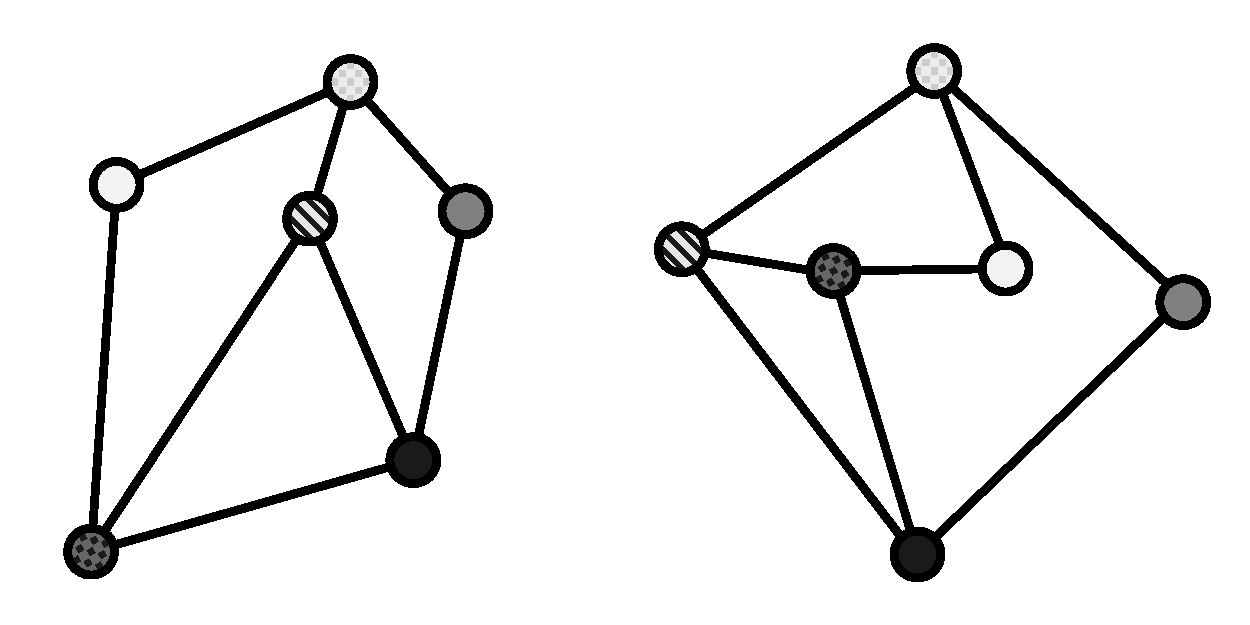
\includegraphics[width=0.7\linewidth]{img/isomorphism-example.pdf}
	\captionof{figure}[Zwei zueinander isomorphe Graphen]{Zwei zueinander isomorphe Graphen. Der Isomorphismus ist durch die gleiche Einfärbung der Knoten visualisiert.}
	\label{fig:isomorphism}
\end{minipage}

\subsubsection{Zero-Knowledge-Beweisprotokoll}

\begin{protocol}[Graphenisomorphismus]
\label{protocol:isomorphism}
Gemeinsame Eingabe: \( G_0 = \left( V_0, E_0 \right) \) und \( G_1 = \left( V_1, E_1 \right) \).\\
Geheime Eingabe an den Beweiser: Isomorphismus zwischen beiden Graphen \( \phi \) mit \( G_0 = \phi \circ G_1 \).
\begin{itemize}
\item[(Beweiser, Schritt 1)] Ziehe zufällige Permutation \( \pi_0 \in S_{\left| V_0 \right| } \) und sende \( G' = \pi_0 \circ G_0 \) an den Verifizierer
\item[(Verifizierer, Schritt 1)] Ziehe zufälliges Bit \( \alpha \in \left\lbrace 0, 1 \right\rbrace \) und sende es an den Beweiser. Implizit bedeutet dies, dass bei \( 0 \) die Permutation \( \pi_0 \) gezeigt werden soll, bei \( 1 \) die Permutation \( \pi_1 \) mit \( G' = \pi_1 \circ G_1 \)
\item[(Beweiser, Schritt 2)] Falls \( \alpha = 1 \), sende \( \pi_1 = \pi_0 \circ \phi \) an den Verifizierer, sonst \( \pi_0 \)
\item[(Verifizierer, Schritt 2)] Akzeptiere, falls \( G' = \pi_\alpha \circ G_\alpha \), sonst verwerfe\footnote{aus \cite[Protocol 2]{np}}
\end{itemize}
\end{protocol}

\subsubsection{Zero-Knowledge-Eigenschaft}

\begin{theorem}
Bei Protokoll \ref{protocol:isomorphism} handelt es sich um ein interaktives Beweissystem.
\end{theorem}

\begin{proof}
Vollständigkeit: Falls \( G_0 \) und \( G_1 \) tatsächlich isomorph sind, kennt \( P \) nach Voraussetzung den Isomporphismus \( \phi \) und kann somit immer sowohl das zufällig gezogene \( \pi_0 \), als auch \( \pi_1 = \pi_0 \circ \phi \) zurückgeben. \\
Korrektheit: Falls \( G_0 \) und \( G_1 \) nicht isomorph zueinander sind, kann \( G' \) nicht isomporph zu beiden Graphen sein - und somit wird \( P \) mit einer Wahrscheinlichkeit \( \geq \frac{1}{2} \) daran scheitern, einen Isomorphismus von \( G_\alpha \) zu \( G' \) anzugeben.
\end{proof}

Höhere Sicherheiten für den Verifizierer als \( \frac{1}{2} \) können dabei durch eine Wiederholung des Beweises (mit einer neuen Permutation) erzielt werden. Nach zehn Beweisen ist man somit beispielsweise bei einer Wahrscheinlichkeit von \( 99,8 \% \).

Dabei sollte nicht zweimal die gleiche Permutation \( \pi_0 \) verwendet werden, da sonst, falls sich der Verifizierer einmal für \( \alpha = 0 \) und einmal für \( \alpha = 1 \) entscheidet, \( \phi \) einfach durch \( \phi = \pi_0^{-1} \circ \pi_1 \) berechnet werden kann.

% TODO: Abstand einfügen
\vspace{0.2cm}

\begin{theorem}
Protokoll \ref{protocol:isomorphism} ist Zero Knowledge.
\end{theorem}

% TODO: Erklärung, warum V* und nicht mit normalen V 

\begin{proof}
\label{proof:zeroisomorphism}
Sei \( V^{\ast} \) eine beliebige, aber feste im Erwartungswert polynomielle ITM. Die Zero-Knowledge-Eigenschaft des Protokolls kann hier konstruktiv bewiesen werden, also durch die Angabe einer im Erwartungswert polynomiellen Maschine \( M_{V^{\ast}} \), die eine rechnerisch ununterscheidbare Verteilung zu einer Kommunikation mit dem Beweiser \( P \) generiert.

Dabei wird \( V^{\ast} \) von einer im Erwartungswert polynomiellen Turing-Maschine \( M_{V^{\ast}} \) simuliert, wobei dieser die Bandinhalte von 
\( M_{V^{\ast}} \) vorgegeben werden.
Das öffentliche Eingabeband von \( V^{\ast} \) ist damit immer mit \( \left( G_0, G_1 \right) \) beschrieben und das geheime Eingabeband bleibt leer. Das Zufallsband von \( V^{\ast} \) wird mit im Voraus von \( M_{V^{\ast}} \) gezogenen Zufallsbits befüllt, die über die gesamte Simulation gleich blieben. Dadurch wird erzielt, dass das Verhalten von \( V^{\ast} \) bei einer erneuten Simulation nur noch von den Inhalten des nur-lesbaren Kommunikationsbandes abhängt, also deterministisch wird.

Um Zero-Knowledge auch bei mehrfacher Ausführung des Protokolls zu beweisen, werden hier mehrere einzelne Ausführungen nacheinander betrachtet. Die Eingaben und Ausgaben von \( V^{\ast} \) über die Kommunikationsbänder werden dabei in einem Kommunikationsprotokoll festgehalten.

Eine einzelne Simulation einer Durchführung des Protokolls beginnt damit, dass \( M_{V^{\ast}} \) ein zufälliges \( \beta \in \left\lbrace 0, 1 \right\rbrace \) und eine zufällige Permutation in \( \psi \in S_{ \left| V_\beta \right| } \) zieht und anschließend damit \( G' = \psi \circ G_\beta \) berechnet. Damit \glqq{}setzt\grqq{} \( M_{V^{\ast}} \) darauf, dass sich \( V^{\ast} \) für \( \beta \) entscheiden wird. Danach wird \( V^{\ast} \) mit allen bisherigen erfolgreichen Durchführungen des Protokolls und zusätzlich dem Beginn des aktuellen (also das Zusenden von \( G' \)) ausgeführt. Falls das von \( V^{\ast} \) gezogene \( \alpha = \beta \) ist, war dieser Beweisschritt erfolgreich und wird dem Kommunikationsprotokoll angehängt, sonst wird die gesamte einzelne Durchführung des Protokolls verworfen und wiederholt. Wenn die gewünschte Anzahl an Einzeldurchführungen erreicht wurde, werden diese zurückgegeben.

Hier lässt sich zeigen, dass die Verteilungen sogar statistisch Zero Knowledge sind, woraus das schwächere rechnerische Zero Knowledge aus Definition \ref{definition:zeroknowledge} folgt.\footnote{Folgerung aus \cite[Seite 193]{identity}. Ein präziserer Beweis, der diesen Beweis zu Ende führt und noch auf einige weitere Details eingeht ist unter \cite[Theorem 2]{np} zu finden.}
\end{proof}

\subsection{Färbung eines Graphen mit drei Farben}
Ein weiteres Entscheidungsproblem mit einem Zero-Knowledge-Beweis ist die Färbung eines Graphen mit drei Farben:

% TODO: Abstand einfügen
\vspace{0.2cm}

\begin{definition}[G3C]
Gegeben sei ein Graph \( G = \left( V, E \right) \). Ein Graph gehört genau dann zu der Sprache der mit nur drei Farben einfärbbaren Graphen \( L_{G3C} \), wenn jedem Knoten eine von drei verschiedenen Farben (in der Definition die Zahlen \( \left\lbrace 1, 2, 3\right\rbrace \)) so zugewiesen werden kann, dass keine Kante zwei Knoten derselben Farbe verbindet.

\[ 
L_{G3C} = \left\lbrace G = \left( V, E \right) \mid \exists \phi: V \rightarrow \left\lbrace 1, 2, 3\right\rbrace: \forall \left( u, v \right) \in E: \phi \left( u \right) \neq \phi \left( v \right) \right\rbrace	
\]
\end{definition}

\vspace{1em}
\begin{minipage}{\linewidth}
	\centering
	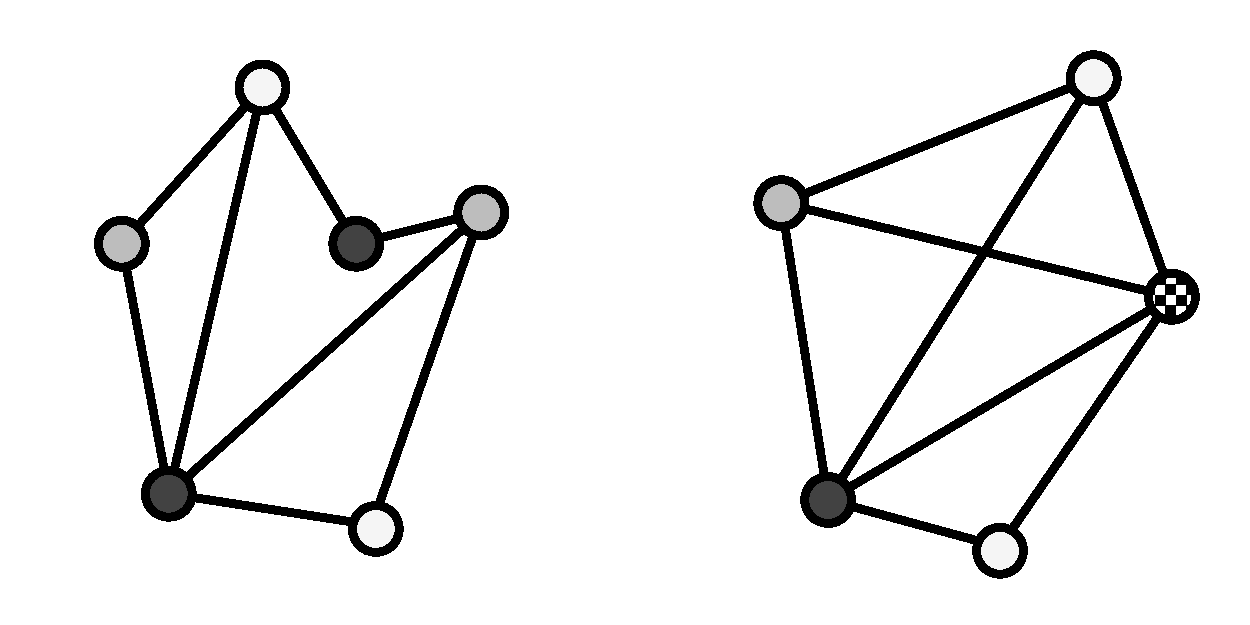
\includegraphics[width=0.7\linewidth]{img/3colorgraphs-example.pdf}
	\captionof{figure}[Beispiel für einen mit drei Farben einfärbbaren (links) und einen nicht mit drei Farben einfärbbaren Graphen (rechts).]{Beispiel für einen mit drei Farben einfärbbaren (links) und einen nicht mit drei Farben einfärbbaren Graphen (rechts).}
	\label{fig:3coloringexample}
\end{minipage}

% TODO: Abstand einfügen
\vspace{0.2cm}

Interessant ist hierbei, dass im Gegensatz zu dem Graphenisomorphismus eine Reduktion von SAT auf die Färbung eines Graphen mit drei verschiedenen Farben exisitert und das Problem damit NP-vollständig ist.\footnote{siehe \cite[Seite 14]{np}} Welche Bedeutung dieser Zero-Knowledge-Beweis somit auf alle Probleme in NP hat, wird nach dem Beweisprotokoll dann in Abschnitt \ref{section:npconsequences} beschrieben. 

\subsubsection{Zero-Knowledge-Beweisprotokoll}
Für diesen Zero-Knowledge-Beweis wird eine sogenannte Einwegfunktion benötigt, mithilfe derer sich der Verifizierer sicher sein kann, dass sich der Beweiser auf einen bestimmten Wert für jeden Knoten festgelegt hat, jedoch nicht auf diese Werte kommen kann. Formal definiert sieht eine solche Funktion wie folgt aus:

\begin{definition}[Einwegfunktion]
Eine Funktion \( f: \left\lbrace 1, 2, 3\right\rbrace \times \left\lbrace 0, 1\right\rbrace ^{\ast} \rightarrow \left\lbrace 0, 1\right\rbrace ^{\ast} \) wird Einwegfunktion genannt, falls folgende Eigenschaften gegeben sind:\footnote{vgl. \cite[Definition 6]{np} und \cite[Definition 2]{20yearszeroknowledge}}

\begin{itemize}
\item[Effiziente Berechenbarkeit:] Die Funktion ist für jede Eingabe in polynomieller Zeit berechenbar.
\item[Kollisionsfreiheit:] \( \forall x, y \in \left\lbrace 1, 2, 3\right\rbrace, x \neq y, r, s \in  \left\lbrace 0, 1\right\rbrace ^{\ast}, r \neq s: f \left( x, r \right) \neq f \left( y, s \right) \)
\item[Sicherheit:] Sei die Zufallsvariable \( f_n \left( x \right) \) definiert als \( f_n \left( x \right) = f \left( x, r_n \right) \) mit jeweils zu\-fäl\-li\-gem \( r_n \in \left\lbrace 0, 1\right\rbrace ^{ n } \) als probabilistische Verschlüsselungsfunktion.
Die Verteilungsfamilien \( \left\lbrace f_n \left( x\right) \right\rbrace_n \) und \( \left\lbrace f_n \left( y\right) \right\rbrace_n \) müssen für alle \( x, y \in \left\lbrace 1, 2, 3\right\rbrace, x \neq y \) rechnerisch ununterscheidbar sein.
\end{itemize}
\end{definition}

Man kann eine Einwegfunktion auch als verschließbare Box ansehen, die vom Beweiser verschlossen an den Verifizierer überreicht wird, der den Inhalt erst dann überprüfen kann, wenn der Beweiser ihm zusätzlich den Schlüssel aushändigt. Der Beweiser kann jedoch, sobald die Box übergeben worden ist, nichts mehr an deren Inhalt ändern.

\begin{protocol}[Kolorierbarkeit mit drei Farben]
\label{protocol:3color}
Gemeinsame Eingabe: \( G = \left( V_G, E_G \right) \).\footnote{aus \cite[Protocol 4]{np}}
Geheime Eingabe an den Beweiser: Korrekte Einfärbung von \( G \): \( \phi : V \rightarrow \left\lbrace 1, 2, 3\right\rbrace \)
\begin{itemize}
\item[(Beweiser, Schritt 1)] Ziehe eine zufällige Permutation \( \pi \) aus \( S_3 \), berechne für jedes \( v \in V_G \) mit einem jeweils eigenen, zufälligen \( r_v \in \left\lbrace 0, 1\right\rbrace ^n \) den Wert \( F_v = f \left( \pi \left( \phi \left( v \right) \right), r_v \right) \) und sende diese
\item[(Verifizierer, Schritt 1)] Ziehe eine zufällige Kante \( \left( u, v \right) \in E \) und sende diese
\item[(Beweiser, Schritt 2)] Falls \( \left( u, v \right) \in E \), schicke dem Verifizierer \( \left( \pi \left( \phi \left( v \right) \right), r_v \right) \) und \( \left( \pi \left( \phi \left( u \right) \right), r_u \right) \)
\item[(Verifizierer, Schritt 2)] Akzeptiere, falls \( F_v \) und \( F_u \) korrekt berechnet worden waren und den beiden verbundenen Knoten unterschiedliche Farben (bzw. hier Zahlen) zugewiesen worden waren, sonst verwerfe
\end{itemize}
\end{protocol}

Der Trick bei diesem Beweis ist, dass dadurch, dass jedes Mal die Farben durch die Permutation \( \pi \) umbenannt werden, der Verifizierer zwar sieht, dass unterschiedliche Farben an zwei benachbarten Knoten verwendet werden, jedoch nicht mehr erfährt, da die Farben zufällig sind.

\vspace{1em}
\begin{minipage}{\linewidth}
	\centering
	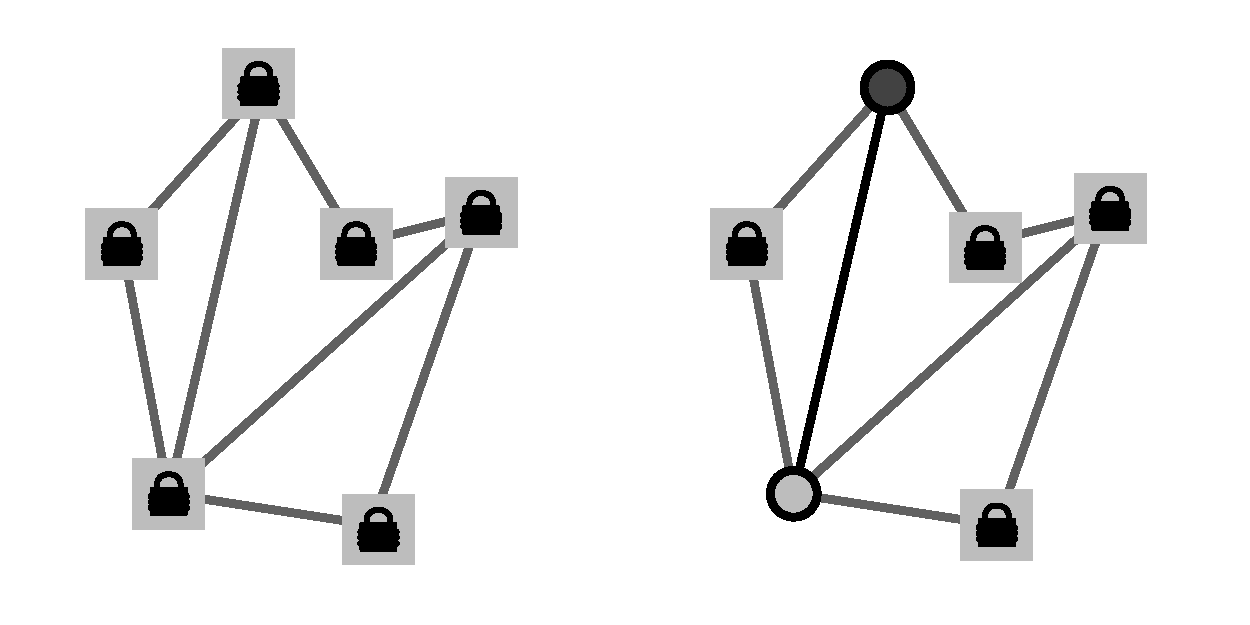
\includegraphics[width=0.7\linewidth]{img/3colorgraphs-proof.pdf}
	\captionof{figure}[Graphische Visualisierung des Beweisprotokolls \ref{protocol:3color}]{Graphische Visualisierung des Beweisprotokolls \ref{protocol:3color}. Links ist zu sehen, was der Beweiser in Schritt 1 sendet, rechts die aufgedeckte Kante aus Schritt 2.}
	\label{fig:3coloringproof}
\end{minipage}

\subsubsection{Zero-Knowledge-Eigenschaften des Beweisprotokolls}

\begin{theorem}
Bei Protokoll \ref{protocol:3color} handelt es sich um ein interaktives Beweissystem.
\end{theorem}

\begin{proof}
Vollständigkeit: Falls \( G \) mit drei Farben einfärbbar ist, kennt \( P \) nach Voraussetzung diese Einfärbung \( \phi \) - und somit kann auch keine Kante entdeckt werden, deren Knoten dieselbe Farbe zugewiesen wurde.\\
Korrektheit: Falls der Graph nicht mit drei Farben korrekt einfärbbar ist, muss es in dem verschlüsselt gesendeten Graphen mindestens eine Kante geben, deren Knoten diesselbe Farbe besitzen. Die Wahrscheinlichkeit dafür, dass diese aufgedeckt wird, beträgt \( \frac{1}{\left| E_G \right|} \). Wie auch im oberen Beweis kann diese Wahrscheinlichkeit durch Mehrfachausführung des Protokolls erhöht werden.
\end{proof}

\begin{theorem}
Bei Protokoll \ref{protocol:3color} ist Zero Knowledge, falls \( f \) eine Einwegfunktion ist.
\end{theorem}

Im Allgemeinen verläuft der Beweis hierzu ähnlich wie bei Satz \ref{proof:zeroisomorphism} - es wird wieder der beliebige Verifizierer \( V^{\ast} \) durch das gleichbleibende Zufallsband deterministisch gemacht und anschließend werdem diesem zufällige Farben für die Knoten verschlüsselt gesendet. Diesmal kann jedoch nur rechnerisches Zero Knowledge (aus Definition \ref{definition:zeroknowledge}) gezeigt werden. Eine Schwierigkeit im Beweis ist, dass der möglicherweise unehrliche Verifizierer seine Entscheidungen auf den verschlüsselten Farben \( \left\lbrace F_v \right\rbrace_{v \in V_G} \) basiert.\footnote{Der vollständige Beweis kann in \cite[Proposition 4]{np} nachgelesen werden.}

\subsection{Folge für alle NP-Probleme}
\label{section:npconsequences}
Da nach \cite{karp} G3C NP-vollständig sind, kann man nun mithilfe der bereits bekannten Reduktionen Zero-Knowledge-Beweise für alle Probleme in NP wie folgt herleiten:

% TODO: Abstand
\vspace{0.2cm}

\begin{theorem}
Falls eine Einwegfunktion exisitiert, besitzt jede Sprache in NP ein interaktives Zero-Knowledge-Beweissystem.
\end{theorem}

\begin{proof}
Sei \( L \) eine beliebige Sprache in \( NP \) und \( g \) eine invertierbare, in polynomieller Zeit ausführbare Reduktion von \( L \) auf SAT. Die ist von jeder Sprache in NP zu (3)SAT durch den Satz von Cook\footnote{siehe \cite{cook}} und mithilfe der Karp-Reduktion\footnote{siehe \cite{karp} als Chromatic Number} weiter zu G3C gegeben. \( g \left( x \right) \) ist somit ein mit drei Farben kolorierbarer Graph.

Bei einer gemeinsamen Eingabe von \( \omega \in L \) berechnen sowohl \( P \) als auch \( V \) den mit drei Farben einfärbaren Graphen \( g \left( \omega \right) \) (und im Falle von \( P\) dessen korrekte Einfärbung)  und führen anschließend den in Protokoll \ref{protocol:3color} gegebenen Beweis aus. Falls dieser erfolgreich ist, akzeptiert \( V \).\footnote{Ein präziserer Beweis ist in \cite[Theorem 5+6]{np} oder \cite[Seite 14]{20yearszeroknowledge} zu finden.}
\end{proof}

\pagebreak

\section{Fiat-Shamir-Identifkationssystem}

Eine naheliegende Verwendung von Zero-Knowledge-Beweisen sind Identifikationssysteme, bei denen ein Verifizierer nicht genug Informationen besitzen darf, um sich selbst gegenüber anderen Verifizierern als der Beweiser ausgeben zu können.\footnote{siehe \cite[Seite 1]{fiatshamir}}

Ein praktisches Szenario davon wäre beispielsweise ein Schlüsselkartensystem, bei dem eine vertrauenswürdige Zentrale (mit hier unbeschränkter Laufzeit) wie die Firmenleitung Schlüsselkarten ausstellt, mit denen sich dann die Mitarbeiter an den Türen verifizieren könnten. Dabei ist es wünschenswert, wenn die Hardware an den Türen möglichst einfach sein kann, also keinen Zugriff auf ein Public-Key-Verzeichnis benötigt und keine aufwendigen Berechnungen durchgeführt werden müssen. Außerdem ist es vorteilhaft, wenn der öffentlich zugängliche Verifizierer keine geheimen Informationen enthält oder verarbeitet, sodass ein Diebstahl oder eine Manipulation des Türöffners dem Angreifer keinen Vorteil bringt. 

In diesem Szenario ist beispielsweise das von Amos Fiat und Adi Shamir entwickelte Identifikationssystem anwendbar, welches im Folgenden vorgestellt wird.

\subsection{Voraussetzungen}

Bevor eine solche Schlüsselkarte ausgestellt werden kann, muss  die Zentrale einmalig zwei geheime Primzahlen \( p \) und \( q \) wählen und deren Produkt \( n = p \cdot q \) veröffentlichen.

Anschließend können Schlüsselkarten, die in der Lage sind, kleine Berechnungen durchzuführen und mit dem Türöffner zu kommunizieren, ausgestellt werden. Auf ihnen sind  die Werte \( v \) und \( s \) gespeichert, die wie folgt berechnet werden können:\footnote{siehe \cite{fiatshamir}. Um das Protokoll zu vereinfachen, habe ich \( k = 1 \) gesetzt und bestimme \( v \) willkürlich.}

% TODO: Abstand
\vspace{0.2cm}

\begin{algorithm}[Ausstellung einer Schlüsselkarte]
\label{algorithm:issue}
Finde ein \( v \in \left\lbrace 1, \dots, n \right\rbrace \), welches ein quadratischer Rest ist, und finde \( v^{-1} \) mit \( v^{-1} \cdot v \textsf{ mod } n = 1 \). Berechne von \( v^{-1} \) die kleinste quadratische Wurzel \( s \) mit \( s^{2} \textsf{ mod } n = v^{-1} \). Stelle die Schlüsselkarte mit \( v \) und \( s \) aus
\end{algorithm}

% TODO: evtl. Quellen einfügen, die begründen, warum diese Werte auch effizient berechenbar sind.

\subsection{Protokoll}
Die Verifizierung der Schlüsselkarte \( P \) an einer Tür \( V \) läuft dann wie folgt ab:

% TODO: Abstand
\vspace{0.2cm}
\begin{protocol}[Verifizierung einer Schlüsselkarte:]
Gemeinsame Eingabe: \( n \) (und gewissermaßen \( v \), da es zu Beginn des Protokolls direkt an \( V \) übertragen wird)\\
Geheime Eingabe an den Beweiser: \( s \)
\label{protocol:fiatshamir}
\item[(Beweiser, Schritt 1)]: Wähle ein zufälliges \( r \in \left\lbrace 0, \dots, n - 1 \right\rbrace \). Sende \( x = r^{2} \) zusammen mit \( v \) an \( V \)
\item[(Verifizierer, Schritt 1)]:  Sende ein zufälliges Bit \( e \in \left\lbrace 0, 1 \right\rbrace \)
\item[(Beweiser, Schritt 2)]: Sende \( y = r \cdot s^e \textsf{ mod } n \)
\item[(Verifizierer, Schritt 2)]: Überprüfe, ob \( x = y^2 \cdot v^e \textsf{ mod } n \)
\end{protocol}

Statt \( v \) willkürlich festzulegen, kann dies auch ein durch einen speziellen \glqq{}Hash-Wert\grqq{} einer von der Zentrale durch die Bestimmung des passenden \(s \) zu signierenden Identifikationszeichenkette festgelegt sein, die dann von der Schlüsselkarte statt \( v \) übertragen wird.

\subsection{Zero-Knowledge-Aspekte}

\begin{theorem}
Bei Protokoll \ref{protocol:fiatshamir} handelt es sich um ein interaktives Beweissystem, wenn \( P \) nicht in polynomieller Zeit die \( \textsf{mod } n \)-Wurzel von \( v \) oder \( v^{-1} \) berechnen kann.
\end{theorem}

\begin{proof}
Vollständigkeit: Falls \( P \) und \( V \) das Protokoll befolgen, akzeptiert \( V \) immer, da \( P \) im Besitz von \( s \) ist und somit das korrekte \( y \) senden kann:
\begin{multline*}
y^2 \cdot v^e \textsf{ mod } n =
\left( r \cdot s^e \right)^2 \cdot v^e \textsf{ mod } n =
r^2 \cdot \left( s^2 \cdot v \right)^e \textsf{ mod } n = \\
\left( r^2 \textsf{ mod } n \right) \cdot \underbrace{ \left( \left( s^2 \cdot v \right)^e \textsf{ mod } n \right) }_{ = 1 \text{ nach Festlegung}} = x
\end{multline*}
Korrektheit: Da sich ein unehrlicher Beweiser \( P \) nicht im Besitz von \( s \) befindet und dieses nach Voraussetzung nicht berechnen kann, muss \( V \) das Bit \( e \) raten - und wird somit mit einer Wahrscheinlichkeit von \( \geq \frac{1}{2} \) enttarnt.\footnote{genauer Beweis ist unter \cite[Lemma 1 + 2]{fiatshamir} zu finden}
\end{proof}

% TODO: Abstand
\vspace{0.2cm}

\begin{theorem}
Protokoll \ref{protocol:fiatshamir} ist Zero Knowledge.
\end{theorem}

Die intuitive Begründung dafür, dass Protokoll \ref{protocol:fiatshamir} Zero Knowledge ist, ergibt sich daraus, dass \( x \) ein Quadrat einer zufälligen Zahl und bei \( y \) das geheime \( s \) durch die Multiplikation mit einer zufälligen Zahl versteckt wird. Somit sind alle Nachrichten, die \( P \) sendet, Zufallszahlen mit einer Gleichverteilung, woran kein unehrlicher Verifizierer \( V^{\ast} \) etwas ändern kann.

Um dies formal zu beweisen, wird wieder ein im Erwartungswert polynomielles \( M_{V^{\ast}} \) angegeben, welches ohne Kenntnis von \( s \) eine von einer echten Ausführung rechnerisch ununterscheidbare Kommunikation generieren kann.\footnote{siehe \cite{fiatshamir}}

% TODO: evtl Cheat-Strategie besprechen

\subsection{Rechenbeispiel}
Um die Funktionsweise des Identifikationsschemas noch einmal zu verdeutlichen, folgt hier ein Zahlenbeispiel mit handlichen Zahlen. In der Orginalarbeit \cite{fiatshamir} von 1986 war für die Praxis ein \( n \) in der Größenordnung von \( 512 \) Bit (statt den \( 4 \) Bit im Beispiel) vorgeschlagen.

\begin{itemize}
\item[Ausstellung durch Zentrale]: In diesem Beispiel seien die geheimen Primzahlen der Zentrale \( p = 3 \) und \( q = 7 \), womit \( n = 21 \). Als \( v \) wurde der Wert \( 16 = 10^2 \textsf{ mod } 21\) gewählt. \( v^{-1} \) ist, damit \( v \cdot v^{-1} \textsf{ mod } 21 = 1 \) erfüllt wird, \( 4 \), womit die \( \textsf{mod } 21 \)-Quadratwurzel \( s \) von \( v^{-1} \) den Wert \( s = 2 \) besitzt.
\item[(Schritt 1)]: Als zufälliges \( r \) zieht der Beweiser \( r = 12 \), womit an den Verifizierer der Wert \( x = r^2 \textsf{ mod } n = 12 ^ 2 \textsf{ mod } 21 = 18 \) gesendet wird. Der Verifizierer zieht daraufhin zufällig \( e = 1 \).
\item[(Schritt 2)]: Der Beweiser antwortet darauf mit \( y = r \cdot s \textsf{ mod } n = 3 \). Der Verifizierer rechnet \( y^2 \cdot v^e \textsf{ mod } n = 3^2 \cdot 16 \textsf{ mod } 21 = 18 = x \), womit der Verifizierer in diesem Beweisdurchgang akzeptiert.
\end{itemize}

\pagebreak


\section{Zerocash}

In den letzten Jahren hat sich die dezentrale Crypto-Währung Bitcoin großer Beliebtheit erfreut. Ein Problem von Bitcoin ist jedoch, dass durch die öffentlichen Transaktionen sowohl die bezahlten Beträge, als auch die Pseudonyme der Nutzer öffentlich sind. Mittlerweile wurden einige Ansätze entwickelt, mit deren Hilfe solche Transaktionen mithilfe der Beträge und des insgesamten Transaktionsgraphen den realen Personen zugeordnet werden können.\footnote{siehe \cite[Seite 3]{zerocash}}

Ein möglicher Ansatz, Daten über Transaktionen geheim und dezentral zu halten ist das Zerocash-Protokoll, das ab 2013 von Kryptographen um Professor Eli Ben-Sasson vom Technion, einem israelischen Institut für Technologie, entwickelt wurde. Zcash wurde als konkrete Implementierung davon am 28. Oktober 2016 von der Zcash Electric Coin Company an den Markt gebracht, die von dem amerikanischen IT-Sicherheitsexperten Zooko Wilcox geleitet wird.\footnote{siehe \cite{nytimeszcash}}

Matthew Green, ein Assistant Professor an der Johns Hopkins-Universität in Maryland, der an der Entwicklung beteiligt war, beschrieb die Motivation hinter Zerocash wie folgt: \glqq{}Während man bei der Verwendung von Bitcoin Spuren hinterlässt, die für immer bleiben werden, soll bei Zcash die Privatsphäre fest im System verankert sein.\grqq{}\footnote{frei übersetzt von \cite{nytimeszcash}}

\subsection{Allgemeiner Aufbau}
Ein Coin besteht aus einer Seriennummer, die bis zum Bezahlen damit privat bleibt und einem geheimen Hintertürchen, aus denen mit einer Einwegfunktion ein sogenanntes Coin-Commitment errechnet wird. Dieses wird in einen öffentlichen Merkle-Baum (einen Baum, bei dem die Eltern eines Knotens mit dem Hash der Kind-Knoten markiert sind) zusammengefasst.

Zerocash benötigt eine einmalige Initialisierung durch einen vertrauenswürdigen Teilnehmer, danach kann die Währung völlig dezentral verwendet werden. Es besitzt wie Bitcoin ein öffentliches, auf mehrere Teilnehmer verteiltes Bestandsbuch (\textit{ledger}), in dem alle Transaktionen eingetragen werden.

Coins können in Zerocash durch die \( \textsf{POUR} \)-Operation aufgebraucht werden, bei dem Coins in andere Coins mit einem anderen Wert \glqq{}umgegegossen\grqq{} werden. Um die korrekte und anonyme Durchführung dieser Akionen zu gewährleisten, werden besondere Zero-Knowledge-Beweise verwendet.

\subsection{zk-SNARKS für \glqq{}Schaltkreise\grqq{}}

Um die Richtigkeit von Ausführungen von Transaktionen zu bestätigen, werden Aussagen über arithmetische Schaltkreise verwendet. Ein arithmetischer Schaltkreis ist ein mathematiches Modell für eine Berechnung mit einem Algorithmus. Die dazu passende NP-Aussage wäre, dass man Eingaben kennt, mit denen der öffentliche arithmetische Schaltkreis zur \( \textsf{POUR} \)-Operation erfüllt werden kann.\footnote{siehe \cite[Seite 5]{zksnark}}

Da es zu aufwendig wäre, wenn jeder Teil des öffentlichen Bestandbuches einen interaktiven Beweis mit dem Urheber der Transaktion führen müsste, wird hier eine andere Art von Zero-Knowledge-Beweisen, die sogenannten Zero Knowledge Succint Non-Interactive Arguments of Knowledge, kurz zk-SNARKs, verwendet.

Argument of Knowledge bedeutet hier, dass im Gegensatz zu den Proofs of Knowledge aus Definition \ref{definition:proofsystem}  die Korrektheit nur gegegenüber polynomiellen unehrlichen Beweisstrategien gewährleistet sein muss.\footnote{siehe \cite[Seite 5]{20yearszeroknowledge}} Mit non-interactive wird gemeint, dass ein Verifizierer nur den Beweis \( \pi \) benötigt, um überzeugt zu werden - eine Interaktion ist nicht nötig. Ein Beweis ist succint, wenn er immer eine konstante Größe besitzt und die Dauer der Überprüfung von der Länge des Eingabewortes abhängt, nicht von der Größe des Schaltkreises. Bei der konkreten Implementierung Zcash ist dabei von wenigen Millisekunden Verifizierungsdauer und einer Größe von einem Bruchteil eines Kilobytes die Rede \footnote{siehe \cite[Seite 5 + 29]{zerocash}} Zero Knowledge sagt in diesem Kontext aus, dass ehrliche Beweise in einem korrekt initialisierten Zerocash-System ununterscheidbar sind von simulierten Beweisen, die von einem mit einem Hintertürchen initialisierten Zerocash-System in polynomieller Laufzeit generiert werden konnten.\footnote{siehe \cite[Seite 11]{zerocash}}

\subsection{POUR-Operation}
Die \( \textsf{POUR} \)-Operation wird verwendet, um Coins in andere Coins umzugießen, und damit Beträge auszuzahlen oder Coins aufzuteilen oder zusammenzuführen.

Die konkrete NP-Aussage ist dabei, dass der Beweiser im öffentlichen Merkle-Baum aufgeführte valide Coins besitzt, die er in andere valide Coins desselben Wertes umgießt.

Zusammen mit unter anderem der Seriennummer des verbrauchten Coins (die dazu dient um Doppelausgaben zu vermeiden) und den Coin-Commitments der entstandenen Coins wird dann der \( \textsf{POUR} \)-Zero-Knowledge-Beweis von den Teilnehmern der öffentlichen Bestandshaltung überprüft und anschließend an diese angehängt.

\subsection{Bewertung}
Innerhalb von wenigen Monaten nach dem Start von Zcash am 28. Oktober 2016 hat es Zcash auf Platz 12 der Kryptowährungen im Bezug auf Marktkapitalisierung geschafft.\footnote{siehe \cite{cryptocurrencymarketcapitalizations}} Auch Edward Snowden soll bei einer Konferenz in Berlin im Videochat Zerocash als verschlüsselte Alternative zu Bitcoin erwähnt haben.\footnote{siehe \cite{snowdenzcash}}

Problematisch bei dem Teil dieser Arbeit war, dass die einzige seriöse Quelle, die ich zu diesem Thema entdecken konnte, die Arbeit zur Entwicklung des Zerocash-Protokolls war, die im Rahmen einer Konferenz veröffentlicht wurden. Dies ist vor allem deshalb kritisch, da die Wissenschaftler, die den Artikel geschrieben haben, an der Zcash Electric Coin Company beteiligt sind, die von jedem erstellten Zcash-Coin \( 10 \% \) \glqq{}Founders Reward\grqq{} bekommen, was bei einem Gesamtwert der im System vorhandenen Coins von 600 Millionen US-Dollar ein beträchtlicher Betrag ist.\footnote{wie im Blogeintrag \cite{zcashfunding} beschrieben.}

\pagebreak


\section{Ausblick}

Eine etwas exotische Anwendungsmöglichkeit von Zero-Knowledge-Beweisen ist die Verifizierung von Atomsprengköpfen für Abrüstungsverhandlungen, wie sie in \cite{nuclear} beschrieben wird.

Um die Einhaltung von Verträgen zu überprüfen, bei denen die maximale Anzahl an Atomsprengköpfen beschränkt wird, wird ein Verfahren benötigt mit dessen Hilfe man testen kann, ob zwei Objekte wie beispielsweise angebliche Nuklearraketen tatsächlich gleich aufgebaut sind. Dabei dürfen jedoch die Inspektoren kein Wissen über den streng geheimen Aufbau erlangen. Genauer gesagt geht es um Messbilder, die durch das Bestrahlen der Sprengköpfe mit hochenergetischen Neutronen entstehen. Der naheliegende Ansatz wäre, ein spezielles Gerät zu konstruieren, welches die Bilder vergleicht und anschließend den Inspektoren nur mitteilt, ob die beiden Konstruktionen ähnlich zueinander sind oder nicht. Problematisch dabei ist, dass sich beide Parteien nicht vertrauen - und die überprüfte Atommacht befürchten muss, durch ein Hintertürchen ausspioniert zu werden; oder die Inspektoren sich nicht sicher sein können, ob das Gerät nicht manipuliert ist. Dies ist vor allem der Fall, da solche Geräte, nachdem sie mit dem klassifizierten Material in Kontakt gekommen sind, nicht weiter durch die Inspektoren überprüft werden dürfen, da sie noch geheime Informationen enthalten könnten.

Mit einem Zero-Knowledge-Beweis ließe sich jedoch dieses Problem lösen. Dabei werden verschiedene Sensorplatten zuerst mit Negativen der zu vergleichenden Testobjekte vorgeladen. Die Inspektoren dürfen dann entscheiden, mit welchen Platten sie welchen Atomsprengkopf messen. Danach wird mit der ausgewählten Platte die Neutronenabstrahlung des ausgewählten Testgeräts aufgenommen. Falls das Vorlageobjekt und das getestete Objekt identisch sind, sieht der Verifizierer nur ein Rauschen und kann mit hoher Wahrscheinlichkeit davon ausgehen, dass beide Objekte identisch sind. Hat die überprüfte Atommacht zwei nicht identische Objekte zum Vergleich angegeben, weichen Teile des Bildes vom normalen Rauschen ab. Dabei sind dann eventuell auch Teile des Aufbaus der Sprengköpfe erkennbar, was den Anreiz ehrlich zu sein erhöhen sollte. Nachdem der Test abgeschlossen ist, kann die Sensorplatte von den Inspektoren weiter überprüft werden, da sie keine geheimen Daten mehr enthält.

Wie hier ersichtlich, ist Idee von Zero-Knowledge-Beweisen also nicht nur für einfache mathematische Konstrukte zu gebrauchen, sondern kann auch in vielen praktischen Gebieten angewendet werden. Da das Gebiet noch relativ neu ist und jährlich neue Erfindung dazukommen, bleibt es spannend, in welchen Bereichen noch Zero-Knowledge-Beweise eingesetzt werden können und welche weiteren theoretischen Ergebnisse präsentiert werden.

\pagebreak


% ----------------------------------------------------------------------------------------------------------
% Literatur
% ----------------------------------------------------------------------------------------------------------
\renewcommand\refname{Quellenverzeichnis}

\bibliographystyle{zeroknowledge_bibliographystyle}
\bibliography{zeroknowledge_bibliography}
\pagebreak

\end{document}

